%This section provides details about the Large Hadron Collider (LHC) and the proton's journey toward the LHC.

The LHC is the most powerful particle accelerator in the world in the present time.
The LHC is a part of the CERN accelerator complex and sits in a tunnel 100 meters underground at CERN, the European Organization for Nuclear Research, on the border of Switzerland and France near Geneva, as shown in Fig.~\ref{fig:LHC_location}.
The LHC ring is quite large, about 27 km in circumference, and it collides hadrons, such as protons or heavy ions, by accelerating them in opposite directions and colliding them.
The CERN accelerator complex is a succession of machines where each machine accelerates a beam of particles to a given energy before injecting the beam into the next machine in the chain.
LHC is the last element of this chain where it is designed to collide particles at the center-of-mass energy up to 14 TeV as shown in Fig.~\ref{fig:acceleration_complex}.

The LHC hosts nine major experiments, each with distinct scientific objectives:
\begin{itemize}
\item {\bf ALICE} – Investigates heavy-ion collisions and quark-gluon plasma (QGP).
\item {\bf ATLAS \& CMS} – Multi-purpose detectors exploring a wide range of physics, including the Higgs boson and new particles.
\item {\bf LHCb} – Focuses on matter-antimatter asymmetry and heavy flavor physics.
\item {\bf LHCf} – Studies forward physics and cosmic ray interactions, sharing an intersection with ATLAS.
\item {\bf TOTEM} – Examines proton-proton scattering, sharing an intersection with CMS.
\item {\bf MoEDAL-MAPP} – Searches for highly ionizing particles and physics beyond the Standard Model, located near LHCb.
\item {\bf FASER} – Detects long-lived particles and neutrinos from LHC collisions.
\item {\bf SND@LHC} – Dedicated to studying neutrinos produced at the LHC.
\end{itemize}

\subsection{The Journey of Protons to the LHC}
The process of producing a beam of protons begins with a compressed hydrogen tank supplying gas to the source chamber of Linear Accelerator 4 (Linac4).
Linac4 accelerates negative hydrogen ions (H$^{-1}$), consisting of a proton with an extra electron, to high energies.
These ions reach speeds of approximately one-third the speed of light ($c$) before being stripped of their electrons.
The resulting protons are then injected into the Proton Synchrotron Booster (PSB), where they undergo further acceleration.

At the Proton Synchrotron Booster (PSB) injection point, a stripping foil removes the electrons from the negative hydrogen ions, converting them into protons.
These protons are then accumulated and organized into beam bunches within the four PSB rings for subsequent acceleration.
These proton bunches are then recombined at the exit of the PSB and further transferred down the CERN injector chain which accelerates the protons up to 91.6\% of $c$.
After that the beam is sent to Proton Synchrotron (PS) where the increase of energy does not transfer to velocity.
Instead, it will increase the relativistic mass accelerating protons up to 99.9\% of $c$. Then the protons are sent to the Super Proton Synchrotron (SPS).

Finally, the LHC features two vacuum pipes, each carrying protons traveling in opposite directions.
The 27 km ring of superconducting magnets keep protons in the ring,
while accelerating structures called radio frequency (RF) cavities boost their energy.
The LHC's RF cavities increase the protons' energy from 450 GeV to 6.5 TeV (1 GeV = 1 billion electron volts).
The maximum energy is reached in around 20 minutes with the bunches having passed through the RF cavities more than 10 million times~\cite{proton}.
There are four locations along the ring where the protons are made to collide.
The CMS experiment is located at one of four collision points, which is the primary focus of this thesis.

 %------------ figures ------------%
\begin{figure}[t!]
\centering
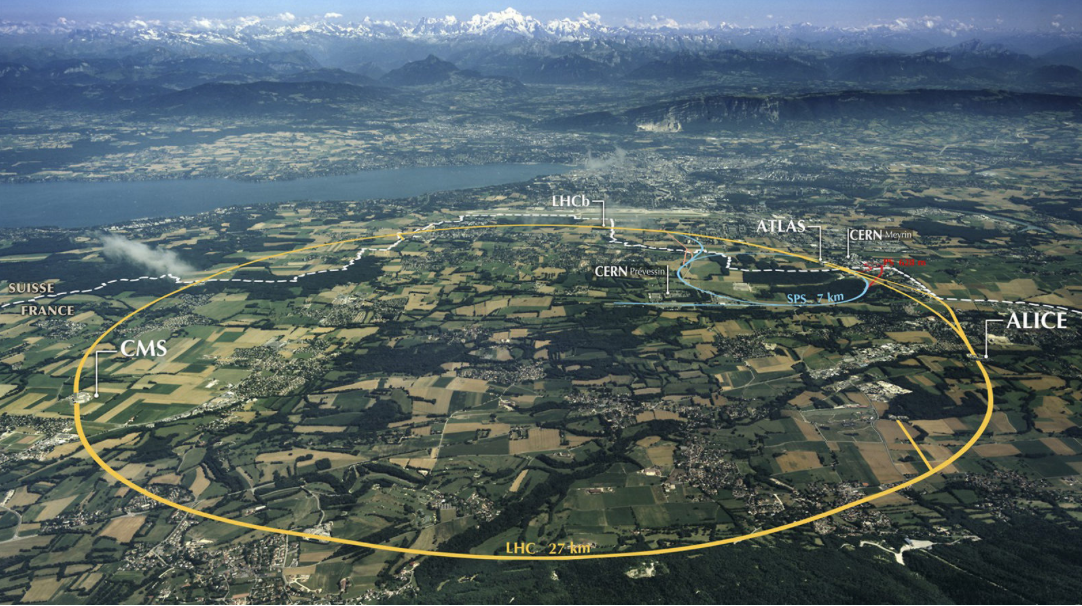
\includegraphics[width=0.99\textwidth]{figures/LHC_location.png}
\caption[A view of the LHC]
{An aerial view of the LHC and the location of its main experiments near the French-Swiss border. Figure source~\cite{LHC_location}.}
\label{fig:LHC_location}
\end{figure}

\begin{figure}[t!]
\centering
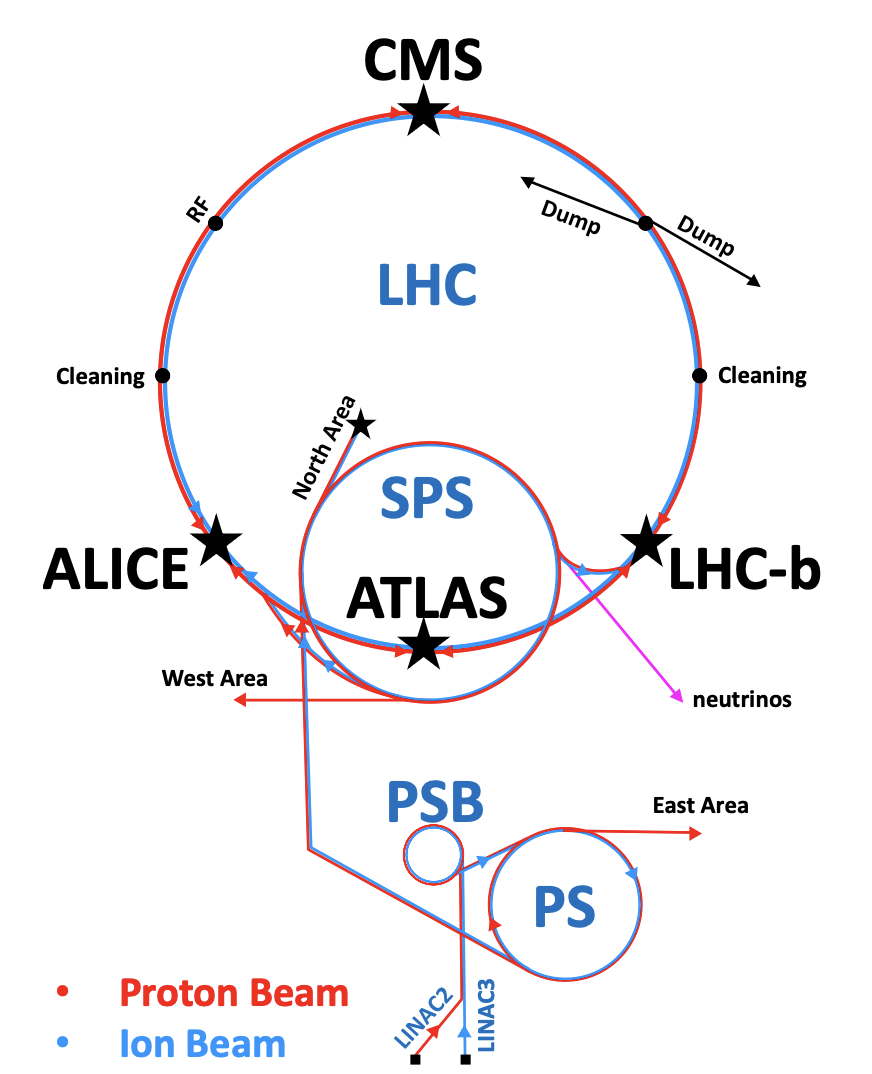
\includegraphics[width=0.75\textwidth]{figures/acceleration_chain.png}
\caption[A diagram of the CERN accelerator chain]
{A schematic diagram of the CERN accelerator chain, including the LINAC, PSB, PS, SPS, and the LHC. The locations of the four main detectors around the LHC are also shown. Figure source~\cite{acceleration_complex}.}
\label{fig:acceleration_complex}
\end{figure}
